\documentclass[a4paper,11pt,abstracton,hidelinks]{scrartcl}

\usepackage[margin=3cm]{geometry}
\usepackage{graphicx}
\usepackage[UKenglish]{babel}
\usepackage{csquotes}
\usepackage[style=numeric,citestyle=numeric,backend=biber,sorting=none,doi=false,url=false]{biblatex}
\usepackage{float}
\usepackage[export]{adjustbox}
\usepackage[T1]{fontenc}
\usepackage{lmodern}
\usepackage[textsize=tiny]{todonotes}
\usepackage[labelsep=period,font=small,labelfont=bf,format=plain]{caption}
\captionsetup[table]{
  position=above,
  belowskip=10pt,
  aboveskip=0pt,
}
\usepackage[group-separator={,}]{siunitx}
\usepackage{booktabs}
\usepackage{pdflscape}
\usepackage{tablefootnote}
\usepackage{authblk}
\usepackage{threeparttable}
\usepackage{afterpage}
\usepackage{lineno}
\linenumbers
\usepackage{setspace}
\usepackage{hyperref}
\doublespacing

\newcommand{\beginsupplement}{%
  \setcounter{table}{0}
  \renewcommand{\thetable}{S\arabic{table}}%
  \setcounter{figure}{0}
  \renewcommand{\thefigure}{S\arabic{figure}}%
}


% TODO create refs.bibmicrosoft 
\addbibresource{refs.bib}


\title{
Genome variation and population structure among 1,142 mosquitoes of the African malaria vector species \emph{Anopheles gambiae} and \emph{Anopheles coluzzii}
}



\author[1]{\small The \emph{Anopheles gambiae} 1000 Genomes Consortium}
\affil[1]{\footnotesize A list of consortium members appears at the end of the paper}

\begin{document}

\maketitle


%%%%%%%%%%%%%%%%%%%%%%%%%%%%%%%%%%%%%%%%%%%%%%%%%%%%%%%%%%%%%%%%%%%%%%%%%%%%%%%
%%%%%%%%%%%%%%%%%%%%%%%%%%%%%%%%%%%%%%%%%%%%%%%%%%%%%%%%%%%%%%%%%%%%%%%%%%%%%%%
\begin{abstract}


%%
Mosquito control remains a central pillar of efforts to reduce malaria burden in sub-Saharan Africa, but insecticide resistance is entrenched in malaria vector populations, and countries with high malaria burden face a daunting challenge to sustain malaria control with a limited set of surveillance and intervention tools. 
%
Here we report on the second phase of a project to build an open resource of high quality data on genome variation among natural populations of the major African malaria vector species \textit{Anopheles gambiae} and \textit{Anopheles coluzzii}. 
%
We analysed whole genomes of 1,142 individual mosquitoes sampled from the wild in 13 African countries, and a further 234 individuals comprising parents and progeny of 11 lab crosses. 
%
The data resource includes high confidence single nucleotide polymorphism (SNP) calls at 57 million variable sites, genome-wide copy number variation calls, and haplotypes phased at biallelic SNPs.
%
We used the SNP data to analyse genetic population structure, compute allele frequencies, and characterise genetic diversity within and between populations.
%
We illustrate the utility of these data by investigating species differences in isolation by distance, genetic variation within proposed gene drive target sequences, and patterns of resistance to pyrethroid insecticides.
%
This data resource provides a foundation for developing new operational systems for molecular surveillance, and for accelerating research and development of new vector control tools.
%%

\end{abstract}


%%%%%%%%%%%%%%%%%%%%%%%%%%%%%%%%%%%%%%%%%%%%%%%%%%%%%%%%%%%%%%%%%%%%%%%%%%%%%%%
%%%%%%%%%%%%%%%%%%%%%%%%%%%%%%%%%%%%%%%%%%%%%%%%%%%%%%%%%%%%%%%%%%%%%%%%%%%%%%%
\section*{Introduction}


%% Need for molecular surveillance. Need for open genomic data resources to underpin surveillance.
%
The 10 countries with the highest malaria burden in Africa account for 65\% of all malaria cases globally, and attempts to reduce that burden are facing significant challenges @@REF.
%
Not least among these, resistance to pyrethroid insecticides is widespread throughout African malaria mosquito populations, potentially compromising the efficacy of mosquito control interventions which remain at the core of global malaria strategy @@REF.
%
There is a broad consensus that further progress cannot be made if interventions are applied blindly, but must instead be targeted and adapted based on data from surveillance of malaria parasite and mosquito populations @@REF.
%
To emphasize this, surveillance is now recommended as a core intervention @@REF, and national surveillance programmes are seeking the capability to capture high resolution molecular data alongside epidemiological and entomological variables.
%
Genome sequencing technologies are widely considered to be a key element of future surveillance systems, and projects are beginning to lay the ground work to enable the scale up and deployment of sequencing technology for public health operations in malaria-endemic countries.
%
These molecular surveillance systems will not work in isolation, but will depend on high quality open genomic data resources, including baseline data on genetic variation from multiple mosquito species and geographical locations, against which comparisons can be made and inferences regarding new events can be drawn.
%%

%% Need to accelerate malaria vector research and development of new vector control tools. Role of open genomic data in accelerating R&D.
%
Better surveillance can increase the impact and longevity of available mosquito control tools, but it is also widely recognised that sustaining malaria control will require the development and deployment of new control tools.
%
This includes repurposing existing insecticides not previously used in public health @@REF, developing entirely new insecticide classes @@REF, and developing tools that don't rely on insecticides, such as attractive toxic sugar baits @@REF and genetic modification of mosquito populations @@REF.
%
Research and development of new mosquito control tools has been greatly facilitated by the availability of open genomic data resources, including high quality genome assemblies and annotations, and more recently by high quality resources on genetic variation among natural mosquito populations @@REFs. 
%
Further expansion of these open data resources to incorporate unsampled mosquito populations and new types of genetic variation can provide new insights into a range of biological and ecological processes, and help to accelerate scientific discovery from basic biology through to operational research.
%%


%% Introduction to Ag1000G. Summary of Ag1000G phase 1. Limitations of Ag1000G phase 1.
%
The Anopheles gambiae 1000 Genomes (Ag1000G) project @@LINK was established in 2013 to build a large scale open data resource on natural genetic variation in malaria mosquito populations.
%
The Ag1000G project forms part of the Malaria Epidemiology Network (MalariaGEN @@LINK), a data-sharing community of researchers investigating how genetic variation in humans, malaria parasites and malaria vectors can inform biology, epidemiology and control of malaria.
%
The first phase of the Ag1000G project released data from whole genome Illumina deep sequencing of mosquitoes from 8 African countries, including SNP calls and phased haplotypes @@REF.
%
Mosquitoes were sampled from a broad geographical range, spanning Guinea-Bissau in West Africa to Kenya in East Africa.
%
Both \textit{Anopheles gambiae} and \textit{Anopheles coluzzii} were sampled, two closely related sibling species within the \textit{Anopheles gambiae} species complex.
%
Genetic diversity was found to be high in nearly all populations, but there were marked patterns of population structure, and clear differences between populations in the magnitude and architecture of genetic diversity, indicating complex and varied demographic histories.
%
However, both of these species have a large geographical range, and many countries and ecological settings are not represented in the Ag1000G phase 1 resource.
%
Also, only SNPs were studied in Ag1000G phase 1, but other types of genetic variation are known to be important.
%
In particular, copy number variation (CNV) has long been suspected to play a key role in insecticide resistance @@REFs, but no previous attempts to call genome-wide CNVs have been made in these species.
%%


%% Introduction to Ag1000G phase 2.
%
This paper describes the data resource produced by the second phase of the Ag1000G project.
%
Within this phase, sampling and sequencing was expanded to include additional wild-caught mosquitoes sampled from five new countries not sampled in phase 1.
%
This includes three new locations with \textit{Anopheles coluzzii}, providing greater power for genetic comparisons with \textit{Anopheles gambiae}, and two island populations, providing a useful reference point to compare against mainland populations.
%
Seven new lab crosses are also included, providing a substantial resource for studying genome variation and recombination within known pedigrees.
%
In this phase we studied both SNPs and CNVs, and rebuilt a haplotype reference panel using all wild-caught specimens.
%
Here we describe the data resource, and use it to re-evaluate major population divisions and characterise genetic diversity.
%
We also illustrate the broad utility of the data by providing some preliminary insights into patterns of pyrethroid resistance; analyse genetic diversity within a gene in the sex-determination pathway currently targeted for gene drive development; and compare geographical population structure between the two mosquito species to investigate evidence for differences in dispersal behaviour.
%%


%%%%%%%%%%%%%%%%%%%%%%%%%%%%%%%%%%%%%%%%%%%%%%%%%%%%%%%%%%%%%%%%%%%%%%%%%%%%%%%
%%%%%%%%%%%%%%%%%%%%%%%%%%%%%%%%%%%%%%%%%%%%%%%%%%%%%%%%%%%%%%%%%%%%%%%%%%%%%%%
\section*{Results}

\subsection*{Population Sampling}
%
In Phase 2 of the Ag1000G Project we sequenced the genomes of 1142 wild caught \emph{Anopheles} mosquitoes; 655 \textit{Anopheles gambiae} individuals, 283 \textit{An. coluzzii} and 204 individuals of undetermined species (individuals with apparent mixed or unclear ancestry).
%
The project now includes 16 distinct populations of mosquitoes, sampled from 13 countries across Sub-Saharan Africa (Figure 1; Table 1). 
%
Single nucleotide polymorphism (SNPs) were identified after read alignment to the AgamP4 reference genome \cite{Holt2002}.
%
We identified accessible regions of the genome; regions in which we can call SNPs with sufficient confidence to be used in analysis of population variation.
%
Inaccessibility may be caused by frequent repeats and consequent mapping errors, copy number variants violating the diploid model, or regions of very high divergence from the reference.
%
Following analysis we defined 61\% (140Mbp) of the genome as accessible, including 91\% (18Mbp) of the exome and 58\% (121Mbp) of non-coding positions.
%
From these genomic regions we identified 57,837,885 high-quality SNPs (an addition of over 5 million variants from Phase 1\cite{Ag1000gConsortium2017}), of which 24\% were classed as multi-allelic (three or more alleles), generating an average of one variant allele every 1.9 bases of accessible genome.
%
Alongside new wild caught sample genomes, Phase 2 also sees the public release of 7 additional lab colony crosses including genomes from both parents and between 14-20 offspring per cross, bringing the total number of available crosses from 4 to 11 (Table \ref{table:colony crosses}).
%
Crosses from lab colonies provide a valuable resource for calibration and validation of population genetic analyses.
%
Whole genome phasing was performed for all samples. 
%
Phasing was evaluated based on successful recovery of haplotypes of cross parents, which were phased by transmission using their progeny.
%%
Quality of phasing varied across the genome. 
%
The overall phasing accuracy rate over the autosomes was 92.2\%, and 89.0\% on the X chromosome.
%
In the autosomes the mean switch distance of 2Mbp regions varied between 26.5kb and 1.7kb, with a median of 2.7kb.
%
On the X chromosome the median switch distance was 3.3kb, with a low of 1.9kb and high of 30.8kbp.
%
Distance between switch errors in the centromeric region was much higher, the 10 windows with the greatest switch distance all appeared after 15Mbp.
%%

\begin{figure}[H]
	\begin{center}
		\includegraphics*[width=5.8in]{artwork/collection_site_map.jpg}
	\end{center}
	\caption{Ag1000G Phase 2 sampling locations. Colour of circle denotes species collected at location and area represents sample size. Colours on the map represent ecosystem classes; dark green designates forest ecosystems; see figure 9 in \cite{sayre2013} for a compete colour legend.}
	\label{sample_map}
\end{figure}


%% Table 1 - Population sampling.
%
\afterpage{%
%\clearpage
% N.B., for some reason using \newgeometry causes page number to get dropped from the subsequent page, so disable for now - not needed if using \footnotesize.
\newgeometry{margin=2cm}
\begin{landscape}
\thispagestyle{empty}
\begin{table}[h]
  \footnotesize
  \centering
  \begin{threeparttable}

  \caption{
%
\textbf{Ag1000G Phase 2 sampling locations}.
}

  \label{table:sampling_locations}

  
\begin{tabular}{lllcccccc}
\toprule
\multicolumn{6}{c}{\textbf{Collection}} &
\multicolumn{3}{c}{\textbf{\emph{Anopheles} species counts}}\\
\cmidrule(r){1-6}
\cmidrule(r){7-9}
Country & 
Location & 
Site &
Year &
Latitude & 
Longitude & 
\emph{gambiae} & 
\emph{coluzzii} & 
Unknown\\
\midrule

Angola & Luanda &  & 2009 & -8.8210 & 13.2910 & 0 & 78 & 0 \\

Burkina Faso & Bana &  & 2012 & 11.2330 & -4.4720 & 20 & 40 & 0 \\

 & Pala &  & 2012 & 11.1500 & -4.2350 & 46 & 10 & 0 \\

 & Souroukoudinga &  & 2012 & 11.2350 & -4.5350 & 26 & 25 & 0 \\

Cameroon & Daiguene &  & 2009 & 4.7770 & 13.8440 & 96 & 0 & 0 \\

 & Gado Badzere &  & 2009 & 5.7470 & 14.4420 & 73 & 0 & 0 \\

 & Mayos &  & 2009 & 4.3410 & 13.5580 & 105 & 0 & 0 \\

 & Zembe Borongo &  & 2009 & 5.7470 & 14.4420 & 23 & 0 & 0 \\

Cote d'Ivoire & Tiassale &  & 2012 & 5.8984 & -4.8229 & 0 & 71 & 0 \\

Equatorial Guinea & Bioko &  & 2002 & 3.7000 & 8.7000 & 9 & 0 & 0 \\

France & Mayotte & Bouyouni & 2011 & -12.7378 & 45.1417 & 1 & 0 & 0 \\

 &  & Combani & 2011 & -12.7787 & 45.1429 & 5 & 0 & 0 \\

 &  & Karihani Lake & 2011 & -12.7965 & 45.1217 & 3 & 0 & 0 \\

 &  & Mont Benara & 2011 & -12.8570 & 45.1552 & 2 & 0 & 0 \\

 &  & Mtsamboro Forest Reserve & 2011 & -12.7027 & 45.0811 & 1 & 0 & 0 \\

 &  & Mtsanga Charifou & 2011 & -12.9907 & 45.1557 & 8 & 0 & 0 \\

 &  & Sada & 2011 & -12.8521 & 45.1039 & 4 & 0 & 0 \\

Gabon & Libreville &  & 2000 & 0.3840 & 9.4550 & 69 & 0 & 0 \\

Gambia, The & Njabakunda & Kerr Birom Kardo & 2011 & 13.5500 & -15.9000 & 0 & 0 & 19 \\

 &  & Kerr Sama Kuma & 2011 & 13.5500 & -15.9000 & 0 & 0 & 8 \\

 &  & Maria Samba Nyado & 2011 & 13.5500 & -15.9000 & 0 & 0 & 18 \\

 &  & Sare Illo Buya & 2011 & 13.5500 & -15.9000 & 0 & 0 & 20 \\

Ghana & Koforidua &  & 2012 & 6.0945 & -0.2609 & 0 & 1 & 0 \\

 & Madina &  & 2012 & 5.6685 & -0.2193 & 12 & 12 & 0 \\

 & Takoradi &  & 2012 & 4.9122 & -1.7740 & 0 & 20 & 0 \\

 & Twifo Praso &  & 2012 & 5.6086 & -1.5493 & 0 & 22 & 0 \\

Guinea & Koraboh &  & 2012 & 9.2500 & -9.9170 & 22 & 0 & 0 \\

 & Koundara &  & 2012 & 8.5000 & -9.4170 & 18 & 4 & 0 \\

Guinea-Bissau & Antula &  & 2010 & 11.8910 & -15.5820 & 0 & 0 & 58 \\

 & Safim &  & 2010 & 11.9569 & -15.6492 & 0 & 0 & 33 \\

Kenya & Kilifi & Junju & 2012 & -3.8620 & 39.7450 & 0 & 0 & 16 \\

 &  & Mbogolo & 2012 & -3.6350 & 39.8580 & 0 & 0 & 32 \\

Uganda & Tororo & Nagongera & 2012 & 0.7700 & 34.0260 & 112 & 0 & 0 \\

\bottomrule
\end{tabular}



  \end{threeparttable}

\end{table}
\end{landscape}
\restoregeometry
} % end afterpage
%% end Table 1


\subsection*{Divergence from the AgamP4 reference genome}

The genomes of \textit{An. coluzzii} and \textit{An. gambiae} samples were similarly diverged from the reference genome used for alignment, AgamP4 \cite{Holt2002}, indicating that unbiased comparisons can be made between the two species based on our results (Fig. \ref{refdiff}a).
%
The similarity in levels of divergence reflect the mixed ancestry of the PEST strain from which the reference genome was derived \cite{Holt2002}.
%
An exception to this is the pericentromeric region of chromosome X, a known region of divergence between the two species \cite{Ag1000gConsortium2017} where the reference genome is closer to \textit{An. coluzzii} than to \textit{An. gambiae}.
%
The similarity of this region to \textit{An. coluzzii} may be due to artificial selection for the X-linked pink eye mutation in the reference strain \cite{Holt2002}, as this originated in the \textit{An. coluzzii} parent it may have led to the removal of any \textit{An. gambiae} ancestry in this region.
%
Reductions in divergence from the reference genome in regions of low recombination are apparent in the centromeres and telomeres, as well as in the large 2La polymorphic inversion in both species \cite{coluzzi2002} (Figure \ref{refdiff}b \& c). 
%
All analyses of geographical population structure were conducted on euchromatic regions of Chromosome 3, which avoids regions of polymorphic inversions, reduced recombination and unequal divergence from the reference genome \cite{Ag1000gConsortium2017}.


\subsection*{Population structure}

Analysis of population structure in the nine Ag1000G Phase 1 populations revealed medically relevant demographic features including connectivity between populations and movement of insecticide resistance mutations across Sub-Saharan Africa \cite{Ag1000gConsortium2017}.
% 
Here we revisit population structure analyses to include the 7 additional populations included in Phase 2.
%%

\begin{figure}[H]
	\begin{center}
		\includegraphics*[width=6.3in]{artwork/main_pca.jpeg}
	\end{center}
	\caption{Principal component analysis of the 1142 wild-caught mosquitoes derived from nucleotide variation in the accessible region of chromosome 3L.}
	\label{pca}
\end{figure}

%
In Phase 1, two of the nine populations were \textit{An. coluzzii} and these, Burkina Faso (BFcol) and Angola (AOcol), were highly differentiated (principal component analysis (PCA), doubleton sharing and F\raisebox{-.4ex}{\scriptsize ST}).
%
This limited our ability to draw general conclusions about the history and population structure of this major malaria vector, and its relationship to its sister species \textit{An. gambiae} difficult to investigate \cite{Ag1000gConsortium2017}.
%
The three additional \textit{An. coluzzii} populations, C\^{o}te d'Ivoire (CIcol), Guinea (GNcol) and Ghana (GHcol) (Figure \ref{sample_map}) are therefore of particular importance to the Phase 2 data release.
%
Substantially less population structure is found between the the three additional Phase 2 \textit{An. coluzzii} populations than between BFcol and AOcol from Phase 1, 
%
PCA analyses found CIcol, GNcol and GHcol clustering together in initial PCA components, BFcol clusters closely but is separated by PC1, with AOcol distant by both PC1 and PC2 (Figure \ref{pca}).
%
Despite the PC1 separation of BFcol from the new \textit{An. coluzzii} samples, doubleton sharing and F\raisebox{-.4ex}{\scriptsize ST}) analyses reveal high sharing and weak allelic differentiation respectively between all \textit{An. coluzzii} populations with the exception of AOcol (Figure \ref{fstdbl}).
%%

\begin{figure}[H]
	\begin{center}
		\includegraphics*[width=6.3in]{artwork/structure_composite.pdf}
	\end{center}
	\caption{\textbf{(a)} Average allele frequency differentiation (F\raisebox{-.4ex}{\scriptsize ST}) between pairs of populations. The bottom left triangle shows average F\raisebox{-.4ex}{\scriptsize ST} values between each population pair. The top right triangle shows the Z score for each F\raisebox{-.4ex}{\scriptsize ST} value estimated via a block-jackknife procedure. \textbf{(b)} Allele sharing in doubleton (\textit{f2}) variants. For each population, we identified the set of doubletons with at least one allele originating from an individual in that population. We then computed the fraction of those doubletons shared with each other population including itself. The height of the coloured bars represent the probability of sharing a doubleton allele between or within populations. Heights are normalized row-wise for each population so that the sum of coloured bars in each row equals 1.
}
	\label{fstdbl}
\end{figure}

%
The Phase 2 Gambian (GM) population is strikingly similar in multiple aspects to the the samples from neighbouring Guinea Bissau (GW).
%
Both populations have similar patterns of ancestry informative marker painting (Figure \ref{aim}), fall together in early principal components (Figure \ref{pca}), show high doubleton sharing with each other but not between other populations (Figure \ref{fstdbl}b) and are weakly differentiated (F\raisebox{-.4ex}{\scriptsize ST} = 0.007 Figure \ref{fstdbl}a).
%
The Phase 2 cohort also includes two \textit{An. gambiae} populations collected from islands, Bioko (GQgam) off the west coast of Africa and Mayotte (FRgam) off the eastern seaboard; despite their island collection our analyses found them highly dissimilar. 
%
GQgam clusters with Ugandan (UGcol), Ghanaian (GHcol) and Cameroonian (CMcol) \textit{An. gambiae} in early PCA components (Figure \ref{pca}), though has elevated levels of genetic differentiation when compared to other 
\textit{An. gambiae vs. An. gambiae} F\raisebox{-.4ex}{\scriptsize ST} values (exluding FRgam) (Figure \ref{fstdbl}a). 
%
FRgam is an outlier in principal components three and four, has almost no doubleton sharing with any other populations and the only population more genetically differentiated in pairwise comparisons is Kenya (KE) which is known to be highly bottlenecked \cite{Ag1000gConsortium2017} (Figure \ref{fstdbl}).
% 
Unlike KE, which appears 'hybridised' in AIM analysis, FRgam is comparable to other An. gambiae populations (Figure S1).
%%


\subsection*{Genetic diversity within populations}

%%
We carried out analyses of the genetic diversity within populations to enable inference of their evolutionary histories.
%
An understanding of historical evolutionary trajectories is essential to parameterise mathematical models and predict future outcomes of vector control methods.
%
%
All but three populations carry similar levels of median genetic diversity (from Guinea \textit{coluzzii} $\pi$ = 0.014 to Guinea \textit{gambiae} $\pi$ = 0.016), with only Angola ($\pi$ = 0.012), Mayotte ($\pi$ = 0.010) and Kenya ($\pi$ = 0.009) presenting lower levels (Figure \ref{div}a).
%
Mayotte and Kenyan samples also stood out in estimations of Tajima's D, which compares the average number of pairwise differences with the number of segregating sites, as the only populations carrying positive median values  (Mayotte Tajima's D = 1.11, Kenya Tajima's D = 1.97 Figure \ref{div}b).
%
The other populations presented Tajima's D values between 0 and -2 (from Angola \textit{coluzzii} D = -0.24 to Cameroon \textit{gambiae} D = -2.058).
%%

%%
Runs of homozygosity present within individuals can be informative with regard to population demography.
%
Both high counts and high fractions of the genome with contiguous runs of homozygosity (ROH) can be indicative of inbreeding.
%
A previous analysis of Phase 1 populations \cite{Ag1000gConsortium2017} saw Kenya stand out with ROH tracts taking up to ~60\% of the genome, a much higher percentage than all other natural populations and similar to individuals from the  Mali lab colony (these were cross parents) (Figure \ref{div}c). 
%
The additional colony cross parents available for analysis in Phase 2 reveal a much broader spread in both count and fraction ROH between colonies, suggestive of different histories.
%
Ghana colony samples appear outbred with similar ROH distributions to wild caught samples, whereas samples from the Kisumu colony have extremely high levels of ROH.    
%%

%%
While the population from Kenya remain an outlier in terms of the high fraction of genomes contained in a ROH, values from the new Phase 2 population from Mayotte were also striking.
%
The island population demonstrates significantly elevated ROH fractions, some samples even matching Kisumu colony's samples with counts of ROH >100, though the ROH were distributed as many smaller regions rather than the large chunks observed in Kenya.
%%

%%
Within population Identity by descent (IBD) was computed across the cohort. 
%
The distribution of IBD can be informative about population demographic history. 
%
As expected given the results above, we see elevated IBD in Kenya, Mayotte, Gabon and Angola (Figure \ref{div}).
%
Compared to other \emph{gambiae} populations, Cameroon shows a large number of small chunks of shared ancestry.
%
Pairs from Cameroon \emph{gambiae} showed a mean of 23 IBD chunks, compared to 11 in the otherwise similar Burkina Faso \emph{gambiae} population.
%
These chunks also tended to be slightly smaller in Cameroon \emph{gambiae} than in Burkina Faso (10.4kb vs 18.3kb). 
%
Such marked differences in IBD between these populations may suggest a distinct population history for Cameroon.
%%


\begin{figure}[H]
	\begin{center}
		\includegraphics*[width=6.3in]{artwork/diversity_composite.jpeg}
	\end{center}
	\caption{Nucleotide diversity (pi)...}
	\label{div}
\end{figure}



%%
The expanded sampling of the phase 2 dataset also allows analysis of fine-scale geographic differentiation among \textit{Anopheles} populations of both \textit{An. gambiae} and \textit{An. coluzzii}.
%
To assess how geographic distance relates to genetic differentiation we calculated Wright's "Neighbourhood Size" \cite{wright1946isolation} for \textit{An. gambiae} and \textit{An. coluzzii} in West Africa (Figure \ref{fig:ibd_fig}a), a measurement of isolation by distance.
%
This statistic is an approximation of the (effective) number of potential mates for an individual and can be viewed as a measure of the strength of isolation by distance - low values indicate strong differentiation across space, and high values weak differentiation.
%
We used Rousset's \cite{rousset1997genetic} method for estimating neighbourhood size based on a regression of normalized $F_{st}$ against the logarithm of geographic distance, and calculated this statistic in 200,000bp windows across the genome for all pairs of localities in western Africa, excluding Angola. 
%
Comparisons were limited to pairs for which both populations belonged to the same species.
%%



\begin{figure}[H]
	\begin{center}
		\includegraphics*[width=6.3in]{artwork/west_africa_multipanel_edit.pdf}
	\end{center}
	\caption{Isolation by distance in west African \textit{Anopheles}. \textbf{(a)} Study region and pairwise $F_{st}$. \textbf{(b)} Regressions of average genome-wide $F_{st}$ against geographic distance, following Rousset \cite{rousset1997genetic}. Neighbourhood size is estimated as the inverse slope of the regression line. \textbf{(c)} Difference in neighbourhood size estimates by species, with each point representing a 200kb region of the genome. \textbf{(d)} Neighbourhood size estimates across the genome, demonstrating heterogeneity relating to inversions (grey bars) and sites implicated in insecticide resistance (black triangles).}
	\label{fig:ibd_fig}
\end{figure}


%%
We found that average neighbourhood sizes are lower in \textit{An. coluzzii} (median=84.7) than in \textit{A. gambiae} (median=260.5; Figure \ref{fig:ibd_fig}b, c), reflecting stronger population structure and potentially lower dispersal in \textit{An. coluzzii} populations.
%
Though both figures are strikingly low relative to census population sizes, our estimate for \textit{A. gambiae} is quite similar to a recent study in a Malaysian population of \textit{An. aegypti} in which neighborhood size was estimated at 268 \cite{jasper2019genomic}.
%
Levels of isolation by distance also vary across the genome in both species (Figure \ref{fig:ibd_fig}d).
%
These patterns appear to reflect the influence of local $N_{e}$ and selection on population differentiation.
%
Deviations from local genomic neighbourhood size coincide with a number of inversions.
%
The large 2La inverted region on chromosome 2L shows a roughly 10-fold drop in neighbourhood size relative to surrounding regions of the genome in both \textit{An. coluzzii} and \textit{An. gambiae}.
%
Dips in estimated neighbourhood sizes were also observed in one or both species near several genes/gene-clusters implicated in insecticide resistance (Figure \ref{fig:ibd_fig}d). 
%%



%% CAS9
\subsection*{Implications for CAS9 gene drive}
%%

In a recent study investigating possibilities of gene drive as a means of vector control, a Cas9 target was designed against a 23bp region spanning an intron-exon boundary that is subject to alternative splicing in the doublesex (\textit{dsx}) gene on chromosome 2R \cite{kyrou2018}.
%
Lack of diversity in the Cas9 target is crucial to the success of this gene drive method, as any variation could inhibit the drive mechanism and thus constitute a resistant genotype that could spread and resist control.
%
This region was found to contain very little genetic diversity, with only one variant site being discovered in the Ag1000G Phase 1 samples \cite{kyrou2018}.
%
We used the Phase 2 dataset to extend the study of diversity in the \textit{dsx} Cas9 target region to more samples and new populations. 
%
No further variant sites were discovered, and the variant allele at the known site was not found in any of the additional populations in phase 2.
%
The mutant allele was present at 2.9\% frequency in Phase 1, and is now at 2.5\% frequency in Phase 2, being found in \textit{An.coluzzii} from Angola (26.5\% frequency), and \textit{An. gambiae} from Cameroon (1.3\%) and Gabon (5.8\%).
%
This site has previously been shown not to interfere with the gene drive process \cite{kyrou2018}, as the guide RNA was able to cleave both the wild-type and the mutant forms of this sequence. 
%
Since we found no other variant sites, there is no evidence from the 1142 samples in Phase 2 of naturally-occurring variation that could disrupt this gene drive target. 

The occurrence of alternative splicing at the site of this gene drive target may explain the low diversity in the region, and could impose purifying selection pressures on a wider area than these 23bp.
%
We investigated variation in the wider region around the target and found that it was lower than the mean variation in other genes on chromsome 2R (\ref{dsx1}). 
%
Diversity was particularly low in the region of the intron near the intron-exon boundary.
%
After removing filtered positions, mean genetic diversity ($\pi$) over the last 100bp of the intron was 0.00046, which was smaller than 99.2\% of comparable introns (at least 300bp in size, with at least 70 of the first 100bp passing filtering) on the chromsome.
%
Diversity in the exon was also low, with $\pi = 0.00055$ over the 92bp of the exon, which is lower than 91.9\% of comparable exons (smaller than 100bp, with at least 70bp passing filtering) on the chromosome. 

%[in case anyone asks, if we only look at the third coding position then about 88\% of exons have higher diversity than this one].


\begin{figure}[H]
	\begin{center}
		\includegraphics*[width=5.5in]{artwork/temp-cas9dsx/Cas9_target_diversity.jpg}
	\end{center}
	\caption{Genetic variation (orange line) around the intron-exon boundary targeted by the gene drive mechanism in \textcite{kyrou2018} is low compared to the average intronic (green bars) or exonic (blue bars) variation on chromosome 2R. Bars show mean and 95\% confidence intervals for each position relative to the start (light blue) or end (green and dark blue) of the genomic feature. To adequately compare with the \textit{dsx} exon and intron plotted here, mean exonic diversity was calculated using exons smaller than 100bp whose first base was the second codon position, and mean intronic diversity was caculated using introns larger than 300bp. Red points indicate positions on the \textit{dsx} gene that were inaccessible and thus where diversity could not be calculated.}
	\label{dsx1}
\end{figure}

\subsection*{Insecticide resistance}
%%

%
An important question currently facing malaria vector control programmes concerns the procurement and deployment of "next-generation" LLINs which combine a pyrethroid with a PBO synergist, counteracting metabolic resistance caused by cytochrome P450 genes \cite{churcher2016, killeen2018, toe2018}.
%
There are no published markers for P450-based pyrethroid resistance, however it is known that P450 resistance can be achieved via over-expression of P450 genes, which in turn can be driven by copy number amplification of the relevant gene within the genome \cite{riveron2014, muller2008}.
%
We scanned the genomes of the mosquitoes in the Phase 2 cohort for evidence of copy number variation, described in more detail in \cite{lucas2019}, these CNV results are released as part of the Phase 2 data resource.
%
At two P450 loci in particular, the \textit{Cyp6p/aa} gene cluster and the \textit{cyp9k1} gene (referred to hereafter as \textit{Cyp6} and \textit{Cyp9} respectively), we found a high frequency of copy number variation in multiple populations.
%
These loci have also been found under recent positive selection in multiple populations \cite{Ag1000gConsortium2017}, and have been associated with mosquito pyrethroid resistance in other studies (\textit{Cyp6} - \cite{nikou2003, edi2014, faucon2015, main2018}, \textit{Cyp9} - \cite{main2018, tchigossou2018, vontas2018}).
%
Thus it is reasonable to assume that the presence of CNVs at these loci is an adaptation to pyrethroids, although this remains to be tested.
%%


%%
We combined the amplification data with data on nucleotide variation within the \textit{Vgsc} gene (Clarkson et al, 2019), the target for pyrethroids, to provide an estimate for the population frequencies of mosquitoes carrying some form of \textit{kdr} target-site pyrethroid resistance, amplifications at either of the two P450 loci, or both (Figure \ref{ir}). 
%
PBO impregnated nets may only offer benefits over traditional LLINs where metabolic resistance to pyrethroids is present at appreciable frequencies.
%
Our analysis reveals several features of the pyrethroid resistance landscape that could determine the effectiveness of PBO bed-nets and therefore inform national malaria control programmes (NMCPs) with respect to bed-net roll-out.
%%


%%

\begin{figure}[H]
	\begin{center}
		\includegraphics*[width=6.3in]{artwork/pyrethroid_resistance_simplified.jpg}
	\end{center}
	\caption{Pyrethroid resistance genotypes. The geographical distribution of four pyrethroid insecticide resistance genotype states for all 1142 Phase 2 wild caught mosquitoes are shown by country across Sub-Saharan Africa. The four pie chart colours represent geneotype state: purple - these individuals were either homozygous or heterozygous for at least one of the two widespread \textit{kdr} pyrethroid target site mutations \textit{Vgsc-995F/S}; yellow - these individuals carried any duplication within genes contained in either the \textit{Cyp6} or \textit{Cyp9} gene clusters; orange - these individuals carried at least one \textit{kdr} mutation and one \textit{Cyp} cluster duplication; grey - these individuals carried no known pyrethroid resistance genotypes (no \textit{kdr} or \textit{Cyp} duplications).}
	\label{ir}
\end{figure}
%%


%%
In West Africa, P450 amplification frequency appears geographically clustered and therefore the potential impact of a PBO bed-net over a traditional LLIN may be regionally described (Figure \ref{ir}).
%
In the "Far-West" populations of Guinea Bissau and The Gambia \cite{caputo2011}, no known \textit{kdr} mutations are detected, however many individuals carry P450 amplifications (in Guinea Bissau 58\% samples carry a P450 amplification, The Gambia 11\%); 
%
a result which suggests PBO net roll-out may be highly advantageous, particularly in Guinea Bissau.
%
The individuals sampled from Guinea, Burkina Faso and C\^{o}te d'Ivoire have high levels of \textit{kdr} mutations but also the highest frequencies of P450 amplifications (Guinea 84\%, Burkina Faso 93\%, C\^{o}te d'Ivoire 97\%), therefore the addition of PBO may increase the level of protection bed-nets provide.
%
Further east, in samples from Gabon, Cameron, Angola and Ghana, lower frequencies of P450 amplification (Gabon 1\%, Cameroon 7\%, Angola 15\%, Ghana 27\%), alongside high \textit{kdr} frequencies, suggest the net gain of PBO inclusion may be small.
%
Eastern populations appear split by the rift valley system, with Uganda presenting high frequencies of P450 mutations (81\%), and therefore the potential for PBO gains, whereas Kenya has almost no P450 amplification (4\%) (Figure \ref{ir}).
%
On the two island population of Bioko and Mayotte no pyrethroid resistance, target-site or metabolic, markers are detected.
%%



%%%%%%%%%%%%%%%%%%%%%%%%%%%%%%%%%%%%%%%%%%%%%%%%%%%%%%%%%%%%%%%%%%%%%%%%%%%%%%%
%%%%%%%%%%%%%%%%%%%%%%%%%%%%%%%%%%%%%%%%%%%%%%%%%%%%%%%%%%%%%%%%%%%%%%%%%%%%%%%
\section*{Discussion}


%%
In this paper we have given an overview of Ag1000G Phase 2, a data release consisting of deep-sequenced whole genome variation from 1142 wild caught \emph{Anopheles} mosquitoes.
%
Genomic variation and meta-data are now available to download via FTP from www.malariagen.net for 16 distinct populations of mosquitoes, sampled from 13 countries across Sub-Saharan Africa. 
%
We defined 61\% (140Mbp) of the genome to be accessible (where we confidently call SNPs) and from these accessible regions we identified 57,837,885 high-quality SNPs, an average of one variant allele every 1.9 bases of accessible genome.
%
Ag1000G Phase 2 also sees the release of data from the parents and offspring of 11 colony crosses, we used the Mendelian errors detectable from parent offspring trios in the quality control process for wild caught samples but these also provide a valuable resource in calibration and validation of population genetic analyses more generally.
%%


%%
For ease of access and research, these data have been released in various analysis-ready formats.
%
Genotype calls for wild caught and lab colony samples are released in three data storage formats, VCF, HDF5 and Zarr, widely accepted as input types for population genomic software.
%
Due to the high diversity of \textit{Anopheles gambiae} and \textit{coluzzii}, raw genotype call files may be prohibitively large in some situations, for this reason we have also released these data in three versions (each in the three data formats): 
%
"raw" data containing all genotype calls, "pass" data containing calls that pass our hard filtering regime from accessible regions of the genome and "biallelic" data, potentially the most useful as both the smallest and the standard input for most population genetic analyses.
%
Biallelic data are the subset of pass data where variants have two alleles, a reference allele and a single alternative allele.
%
In Phase 2 this subset consists of 44,076,901 SNPs.
%
Whole genome phasing was performed using these biallelic variants, estimating chromosomal haplotypes for each sample, a data resource useful for many population genetic analyses including scans for selection.
%
Alongside meta-data for each sample containing details on where and when the sample was collected we have also added presence/absence information for known insecticide resistance loci.
%
These meta-data will therefore allow quick and easy access to population resistance frequencies without requiring bioinformatic tools. 
%%


%%
As evidenced by the research made possible through the first phase of Ag1000G \cite{Ag1000gConsortium2017} (\textit{e.g.} selection scans \cite{xue2019} and demographic modelling \cite{khatri2018}), this newly expanded genomic resource holds a huge potential for furthering our understanding of mosquito evolution and improving vector control.
%
While describing this data release using population genetic measures of diversity and structure we show that, when applied genome-wide, these measurements can reveal medically relevant characteristics.
%
The expanded geographical sampling of Phase 2 allowed fine-scale analysis of how geographic distance between populations is related to genetic distance (isolation by distance), enabling inference of mosquito migration.
%
These analyses found much lower isolation by distance in \textit{An. gambiae} than \textit{An. coluzzii}, suggesting long distance gene flow, and therefore long distance migration in the former but not the latter species (concordant with conclusions made from the results of a study using time-series analyses \cite{dao2014}).
%
The higher genetic connectivity found in \textit{An. gambiae}, compared with \textit{coluzzii}, has important connotations for CRISPR Cas9 gene-drive mediated vector control as high migration in \textit{gambiae} may make these populations more susceptible to introgression of gene-drive resistance loci.
%
Gene-drive resistance can be caused by genetic diversity in the Cas9 binding target, natural variation here could inhibit the drive mechanism and thus constitute a resistant genotype that could spread and resist control (@@best ref?).
%
A gene-drive construct targeting the \textit{dsx} gene has already been proposed for release into natural populations \cite{kyrou2018}.
%
Using the Phase 2 resources, we found no evidence of novel naturally-occurring variation that could disrupt Cas9 binding.
%%


%%
We also utilised the deep-sequencing and broad geographic coverage of these data to demonstrate a genomic approach to insecticide resistance management.
%
With the reliance on pyrethroid insecticides for ITNs and the ubiquity of pyrethroid resistance \cite{Hemingway2016}, it is essential for NMCPs to be able to access information about which regions might benefit from new (and more expensive \cite{churcher2016}) PBO bed-nets.
% 
By combining genomic data on loci associated with pyrethroid target-site and metabolic resistance, we were able to create a snapshot of putative resistance topology across Africa.
%
Results revealed that resistance topology fell broadly into three types (Figure \ref{ir}), each informative to the potential impact of PBO nets on vector populations:
%to vector control
\textbf{1.} Regions with only metabolic pyrethroid resistance alleles, where the PBO nets may drastically reduce the resistance phenotype.
%
\textbf{2.} Regions with both high target-site and high metabolic pyrethroid resistance associated loci frequencies, in these regions many individuals carry markers for both modes of resistance.
%to vector control
The outcome of PBO nets is harder to predict in these regions, as the addition of the synergist can only reduce the metabolic resistance mediated fraction of the pyrethroid resistance phenotype.
%
\textbf{3.} Regions with low frequency or no markers for metabolic resistance, here the combination of low potential benefits and the increased cost of the nets may render distribution inadvisable.
%%

%%
It must be reiterated that these results, though informative, are a prediction of pyrethroid resistance at the time of sample collection (Table \ref{table:sampling_locations}).
%
It is also likely that the four loci we analysed do not explain all phenotypic variation in all locations \cite{donnelly2016, mitchell2014} and, although all loci involve resistance associated genomic regions, the specific P450 CNVs used here have yet to undergo molecular validation \cite{lucas2019}.
%
In order to extract the maximum value from future genomic insecticide resistance monitoring we suggest a two stage approach.
%
Firstly, sampling should be conducted on a wider geographic scale, to improve understanding of population structure and diversity across sub-Saharan Africa, ensuring that genetically representative sentinel collection sites can be chosen and established.
%
Baseline frequencies for known resistance associated loci can then be established and putative resistance loci validated.
%
Secondly, samples should be collected regularly from sentinel sites across Africa, changes in frequencies of resistance associated loci can then be detected and this information can be quickly relayed to stakeholders to inform vector control programs.
%
This temporal genomic sampling also allows detection of new loci potentially linked to resistance by monitoring changes in frequency of alleles across the whole genome.
%%

%%
MalariaGen is committed to sequencing and releasing data that will make this approach to genomic insecticide resistance surveillance possible. 
%
Phase 3 of Ag1000G will see genome sequencing and related meta data released for @@n natural populations of \textit{Anopheles gambiae}, \textit{coluzzii} and \textit{arabiensis}, from @@n countries, filling gaps in current coverage including populations from central Africa.
%
The successor to Ag1000G, the Vector Observatory plans on sequencing 40,000 wild caught mosquitoes collected at sentinel sites across the world in both temporal and spatial transects.
%
These data will be curated and released in the same format as Ag1000G, generating unparalleled resources for vector management tools including genomic surveillance. 
%%


%%
Here, in this brief overview of Ag1000g Phase 2, we provide examples of how this rich resource of deep genome sequencing data can quickly, easily and relatively cheaply edify gene-drive vector control development, PBO net distribution and insecticide choice.
%
Our findings emphasize the value of large publicly available genomic data that can inform many aspects of malaria control while filling gaps in our understanding of mosquito evolution and elucidating basic biological/ecological processes.
%
Expanding and improving these repositories with higher sampling coverage and faster data turnaround can only strengthen the vector control armamentarium in the fight against malaria.
%%

%%%%%%%%%%%%%%%%%%%%%%%%%%%%%%%%%%%%%%%%%%%%%%%%%%%%%%%%%%%%%%%%%%%%%%%%%%%%%%%
%%%%%%%%%%%%%%%%%%%%%%%%%%%%%%%%%%%%%%%%%%%%%%%%%%%%%%%%%%%%%%%%%%%%%%%%%%%%%%%
\section*{Methods}


%%%%%%%%%%%%%%%%%%%%%%%%%%%%%%%%%%%%%%%%%%%%%%%%%%%%%%%%%%%%%%%%%%%%%%%%%%%%%%%
\subsection*{1. Population sampling}

%
Ag1000G Phase 2 mosquitoes were collected from natural populations at 33 sites from 23
geographical locations in 13 sub-Saharan African countries. 
%
Samples have been grouped into 16 populations based on collection country and species (Figure \ref{sample_map} \& Table \ref{table:sampling_locations}).
%
Throughout, we use species nomenclature following Coetzee \textit{et al}. \cite{Coetzee2013};	
%
prior to	 Coetzee	 \textit{et al}., \textit{An. gambiae} was known as \textit{An. gambiae sensu stricto} (S form) and \textit{An. coluzzii} was known as \textit{An. gambiae sensu stricto} (M form).
%
Details of the eighteen collection sites novel to Ag1000G Phase 2 (dates, collection and DNA extraction methods) can be found in the Methods section.
%
Information pertaining to the collection of samples released as part of Ag1000G Phase 1 can be found in the supplementary methods of Ag1000G Consortium (2017) \cite{Ag1000gConsortium2017}.
%
Unless otherwise stated, the DNA extraction method used for the collections described below was Qiagen DNeasy Blood and Tissue Kit (Qiagen Science, MD, USA).
%%

%%%%%%%%%%%%%%%%%%%%%%%%%%%%%%%%%%%%%%%%%%%%%%%%%%%%%%%%%%%%%%%%%%%%%%%%%%%%%%%
\subsection*{1.1 Novel Phase 2 natural populations}
%
\textbf{C\^{o}te d'Ivoire (CIcol)}: Tiassal\'{e} (-4.823, 5.898) is located in the evergreen forest zone of southern C\^{o}te d'Ivoire.
%
The primary agricultural activity is rice cultivation in irrigated fields.
%
High malaria transmission occurs during the rainy seasons, between May and November.
%
Samples were collected as larvae from irrigated rice fields by dipping between May and Septermber 2012.
%
All larvae were reared to adults and females preserved over silica for DNA extraction.
%
Specimens from this site were all \textit{An. coluzzii}, determined by PCR assay \cite{Santolamazza2008}
%%

\textbf{Bioko Island - Equatorial Guinea (GQgam)}: Collections were performed during the rainy season in September, 2002 by overnight CDC light traps in Sacriba of Bioko island (8.7, 3.7).
%
Specimens were stored dry on silica gel before DNA extraction.
%
Specimens contributed from this site were \textit{An. gambiae} females, genotype determined by two assays \cite{Scott1993, Santolamazza2004}.
%
All specimens had the 2L\textsuperscript{+a}/2L\textsuperscript{+a} karyotype as determined by the molecular PCR diagnostics \cite{White2007}. 
%
These mosquitoes represent a population that inhabited Bioko Island before a comprehensive malaria control intervention initiated in February 2004 \cite{Sharp2007}. 
%
After the intervention \textit{An. gambiae} was declining, and more recently almost only \textit{An. coluzzii} can be found \cite{Overgaard2012}.
%%

%
\textbf{Mayotte Island - France (FRgam)}: Samples were collected as larvae during March-April 2011 in temporary pools by dipping, in Bouyouni (-12.738, 45.143), M'Tsamboro Forest Reserve (-12.703, 45.081), Combani (-12.779, 45.143), Mtsanga Charifou (-12.991, 45.156), Karihani Lake forest reserve (-12.797, 45.122), and Sada (-12.852, 45.104) in Mayotte island.
%
Larvae were stored in 80\% ethanol prior to DNA extraction. 
%
All specimens contributed to Ag1000G Phase 2 were \textit{An. gambiae} \cite{Santolamazza2004} with the standard 2L\textsuperscript{+a}/2L\textsuperscript{+a} or inverted 2L\textsuperscript{a}/2L\textsuperscript{a} karyotype as determined by the molecular PCR diagnostics \cite{White2007}.
%
The samples were identified as males or females by the sequencing read coverage of the X chromosome using LookSeq \cite{Manske2009}.
%%

%
\textbf{The Gambia (GM)}: Indoor resting female mosquitoes were collected by pyrethrum spray catch from four hamlets around Njabakunda (-15.90, 13.55), North Bank Region, The Gambia between August and October 2011.
%
The four hamlets were Maria Samba Nyado, Sare Illo Buya, Kerr Birom Kardo, and Kerr Sama Kuma; all are within 1 km of each other.
%
This is an area of unusually high hybridization rates between \textit{An. gambiae s.s.} and \textit{An. coluzzii} \cite{Caputo2008, Nwakanma2013}.
%
Njabakunda village is approximately 30 km to the west of Farafenni town and 4 km away from the Gambia River.
%
The vegetation is a mix of open savannah woodland and farmland.
%
With apparent high gene-flow in the region, it is problematic to assign species to these samples.
%%

%
\textbf{Ghana (GHcol/GHgam)}: Twifo Praso (5.609, -1.549) a peri-urban community located in semi-deciduous forest in the Central Region of Ghana.
%
It is an extensive agricultural area characterised by small-scale (vegetable growing) and large-scale commercial farms such as oil palm and cocoa plantations.
%
Mosquito samples were collected as larvae from puddles near farms between September and October, 2012.
%
Madina (5.668,	-0.219) is suburb of Accra within a coastal savanna zone of Ghana. 
%
It is an urban community characterised by myriad vegetable-growing areas.
%
The vegetation consists of mainly grassland interspersed with dense short thickets often less than 5 m high with a few trees.
%
Specimens were sampled from puddles near roadsides and farms between October and December 2012.
%
Takoradi (4.912, -1.774) is the capital city of Western Region of Ghana.
%
It is an urban community located in the coastal savanna zone.
%
Mosquito samples were collected from puddles near road construction and farms between August and September 2012.
%
Koforidua (6.094, -0.261) is a capital city of Eastern Region of Ghana and is located in semi-deciduous forest. 
%
It is an urban community characterized by numerous small-scale vegetable farms. 
%
Samples were collected from puddles near road construction and farms between August and September 2012.
%
Larvae from all collection sites were reared to adults and females preserved over silica for DNA extraction.
%
Both \textit{An. gambiae} and \textit{An. coluzzii} were collected from these sites, determined by PCR assay \cite{Santolamazza2008}.
%%

%
\textbf{Guinea-Bissau (GW)}: Mosquitoes were collected in October 2010 using indoor CDC light traps, in the village of Safim (11.957, -15.649), ca. 11 km north of Bissau city, the capital of the country.
%
Malaria is hyperendemic in the region and transmitted by members of the Anopheles gambiae complex (Vicente et al., 2017).
%
\textit{Anopheles arabiensis, An. melas, An. coluzzii} and \textit{An. gambiae}, as well as hybrids between the latter two species, are known to occur in the region \cite{Gordicho2014, Vicente2017}.
%
Mosquitoes were preserved individually on 0.5ml micro-tubes filled with silica gel and cotton. DNA extraction was performed by a phenol-chloroform protocol \cite{Donnelly1999}.
%
Guinea-Bissau is another region where defining species is problematic (Vicente), so no species has been assigned here.
%%

%%%%%%%%%%%%%%%%%%%%%%%%%%%%%%%%%%%%%%%%%%%%%%%%%%%%%%%%%%%%%%%%%%%%%%%%%%%%%%%
\subsection*{1.2 Colony populations}

%%
The Ag1000G Phase 2 data release includes the genomes of seven additional lab colony crosses, both parents and offspring (Table \ref{table:colony crosses}):
%
cross 18-5 (Ghana mother x Kisumu/G3 father, 20 offspring); 37-3 (Kisumu x Pimperena, 20 offspring); 45-1 (Mali x Kisumu, 20 offspring); 47-6 (Mali x Kisumu, 20 offspring); 73-2 (Akron x Ghana, 19 offspring); 78-2 (Mali x Kisumu/Ghana, 19 offspring); 80-2 (Kisumu x Akron, 20 offspring).
%
Father colonies with two names, \textit{e.g.} "Kisumu/G3", signify that the father is from one of these two colonies, but exactly which one is unknown.
%
The	colony labels, \textit{e.g.}	"18-5", are	identifiers used for	
each of the crosses	within the project and	have no special meaning.	
%
Information pertaining to the crosses released as part of Ag1000G Phase 1 can be found in the supplementary methods of Ag1000G Consortium (2017) alongside methods for cross creation and processing. \cite{Ag1000gConsortium2017}.
%%

%%%%%%%%%%%%%%%%%%%%%%%%%%%%%%%%%%%%%%%%%%%%%%%%%%%%%%%%%%%%%%%%%%%%%%%%%%%%%%%
\subsection*{2 Whole genome sequencing}

%
Sequencing was performed on the Illumina HiSeq 2000 platform at the Wellcome Trust Sanger Institute.
%
Paired-end multiplex libraries were prepared using the manufacturer's protocol, with the exception that genomic DNA was fragmented using Covaris Adaptive Focused Acoustics rather than nebulization.
%
Multiplexes comprised 12 tagged individual mosquitoes and three lanes of sequencing were generated for each multiplex to even out variations in yield between sequencing runs.
%
Cluster generation and sequencing were undertaken per the manufacturer's protocol for paired-end 100 bp sequence reads with insert size in the range 100-200 bp.
%
Target coverage was 30X per individual.
%%


\subsection*{2.1 Genome accessibility}

%
For various population-genomic analyses, it is necessary to have a map of which positions in the reference genome can be considered accessible (in which we can confidently call genetic variation).
%
For Phase 2 we repeated the Phase 1 acccessibility analyses \cite{Ag1000gConsortium2017} with 1142 samples and the additional Mendelian error information provided by the 11 crosses (in Phase 1 there were four crosses).
%
Following these analyses it was apparent that the Phase 1 accessibility classifications were also appropriate in application to Phase 2.
%
Reference genome positions were accessible if: 
Not repeat masked by DUST; 
No Coverage <= 0.1\% (at most 1 individual had zero coverage); 
Ambiguous Alignment <= 0.1\% (at most 1 individual had ambiguous alignments); 
High Coverage <= 2\% (20 individuals); 
Low Coverage <= 10\% (114 individuals); 
Low Mapping Quality <= 10\% (114 individuals).
%%

\subsection*{2.2 Sequence analysis and variant calling}
%
Sequencing pipelines were unchanged from Phase 1 of the Anopheles 1000 genomes project\cite{Ag1000gConsortium2017}.
%
Briefly, sequence reads were aligned to the AgamP3 reference genome \cite{sharakhova2007update} using \texttt{bwa v0.6.2}, duplicate reads marked \cite{li2009} and SNPs discovered using \texttt{GATK Unified Genotyper 2.7.4} \cite{van2013} following best practice recommendations. 
%%


\subsection*{2.3 Variant Filtering}
%
Following Ag1000G Phase 1 \cite{Ag1000gConsortium2017}, we applied the following SNP filters to reduce the number of false SNP discoveries.
%
We filtered any SNP that occurred at a genome position classified as inaccessible as described in the section on genome accessibility above, thus removing SNPs with evidence for excessively high or low coverage or ambiguous alignment. 
%
We then applied additional filters using variant annotations produced by GATK based on an analysis of Mendelian error in all 11 crosses present in Phase 2 and Ti/Tv ratio similar to that described above for the genome accessibility analysis.
%
We filtered any SNP that failed any of the following criteria: QD <5; FS >100; ReadPosRankSum <-8; BaseQRankSum <-50. 
%%


%
Of 105,486,698 SNPs reported in the raw callset, 57,837,885 passed all quality filters, 13,760,984 (23.8\%) of which were multi-allelic (>= 3 alleles).
%
To produce an analysis-ready VCF file for each chromosome arm, we first removed all non-SNP variants. 
%
We then removed genotype calls for individuals excluded by the sample QC analysis described above, then removed any variants that were no longer variant after excluding individuals. 
%
We then added INFO annotations with genome accessibility metrics and added FILTER annotations per the criteria defined above. 
%
Finally, we added INFO annotations with information about functional consequences of mutations using SNPEFF version 4.1b \cite{Cingolani2012}.
%%


\subsection*{2.4 Sample quality control}
%
A total of 1285 individual mosquitoes were sequenced as part of Ag1000G phase 2 and included in the cohort for variant discovery. 
%
After variant discovery, quality-control (QC) steps using coverage and contamination filters alongside principal component analysis and meta data concordance were performed to exclude individuals with poor quality sequence and/or genotype data as detailed in \cite{Ag1000gConsortium2017}.
%
A total of 143 individuals were excluded at this stage, retaining 1142 individuals for downstream analyses.

%%


%%%%%%%%%%%%%%%%%%%%%%%%%%%%%%%%%%%%%%%%%%%%%%%%%%%%%%%%%%%%%%%%%%%%%%%%%%%%%%%
\subsection*{2.5 SNP validation}

We used 11 laboratory crosses, each with between 14-20 progeny, to estimate the error associated with genotyping from short reads. 
%
We defined errors at sites where given confident parental genotypes and Mendelian inheritance, the expected genotypes of progeny are known. 
%
At loci where both parents are homozygous for the reference or alternate allele, we expect the progeny to be homozygous for the reference or alternate allele accordingly.
%
When one parent is homozygous for the reference allele, and the other the alternate allele we expect all progeny to be heterozygous. 
%
Therefore we can generate ascertainment error estimates for heterozygous, homozygous reference and homozygous alternate genotypes.
%
To meet the confidence threshold for homozygous calls, both parents must have 30x coverage, and have no discordant reads.
%
Sites are considered erroneously called if at least 10 progeny have genotypes called at that locus, and one or more do not match the expected genotype. 
%
Sites are considered correctly called if at least 10 progeny have genotypes called and all match the expected genotype. 
%
Error in ascertainment rates are computed over each cross, and errors are reported as the median over all 11 crosses. 
%
%
Raw error rates were 0.72\% (0.39, 2.44) for heterozygotes, 0.07\% (0.03, 0.25) for homozygous reference calls, and 0.82\% (0.37, 1.47) for homozygous alternate calls. 
%
Following variant filtering via QC thresholds and the accessibility map these values dropped to 0.26\% (0.15, 1.23) for heterozygotes, 0.02\% (0.01, 0.12) for homozygous reference calls, and 0.80\% (0.31, 1.51) for homozygous alternate calls. 
%%



%%%%%%%%%%%%%%%%%%%%%%%%%%%%%%%%%%%%%%%%%%%%%%%%%%%%%%%%%%%%%%%%%%%%%%%%%%%%%%%
\subsection*{2.6 Haplotype estimation}

%
Haplotype estimation, also known as phasing, was performed on all Phase 2 wild-caught individuals using unchanged methodology from Phase 1 of the Anopheles 1000 genomes project\cite{Ag1000gConsortium2017}.
%
In short, SHAPEIT2 was used to perform statistical phasing with information from sequence reads.
%
Phasing performance was then evaluated by comparison with haplotypes generated from the laboratory crosses and from male X chromosome haplotypes.
%%

%%%%%%%%%%%%%%%%%%%%%%%%%%%%%%%%%%%%%%%%%%%%%%%%%%%%%%%%%%%%%%%%%%%%%%%%%%%%%%%
\subsection*{3 Population structure}

%
Population structure analyses, AIM, F\raisebox{-.4ex}{\scriptsize ST} and PCA were conducted following methods defined in \cite{Ag1000gConsortium2017}.
%
Doubleton sharing was also conducted following \cite{Ag1000gConsortium2017}, except that due low sample sizes in GHgam (12 samples), GNcol (4) and GQgam (9) were excluded.  
%%


%%%%%%%%%%%%%%%%%%%%%%%%%%%%%%%%%%%%%%%%%%%%%%%%%%%%%%%%%%%%%%%%%%%%%%%%%%%%%%%
\subsection*{4 Genetic diversity}

%
Investigations into and utilising genetic diversity, nucleotide diversity, Tajima's D, ROH and IBD (identity by descent), were conducted following methods defined in \cite{Ag1000gConsortium2017} but using the Phase 2 data release of 1,142 samples.
%
In short, scikit-allel ('1.2.0') was used to calculate windowed averages of nucleotide diversity and Tajima's D \cite{miles2018}, IBDseq version r1206 \cite{browning2015} was used to calculate IBD and an	HMM	implemented	in	Python (available in scikit-allel) was used to calculate ROH.

%%%%%%%%%%%%%%%%%%%%%%%%%%%%%%%%%%%%%%%%%%%%%%%%%%%%%%%%%%%%%%%%%%%%%%%%%%%%%%%
\section*{Authors}

%
\textbf{Data analysis group}: Alistair Miles (project lead), Nicholas J. Harding, Giordano Bott\'{a}, Chris S. Clarkson, Tiago Ant\~{a}o, Krzysztof Kozak, Daniel R. Schrider, Andrew D. Kern, Seth Redmond, Igor Sharakhov, Richard D. Pearson, Christina Bergey, Michael C. Fontaine, Martin J. Donnelly, Mara K. N. Lawniczak and Dominic P. Kwiatkowski (chair).
%%

%
\textbf{Partner working group}: Martin J. Donnelly (chair), Diego Ayala, Nora J. Besansky, Austin Burt, Beniamino Caputo, Alessandra della Torre, Michael C. Fontaine, H. Charles J. Godfray, Matthew W. Hahn, Andrew D. Kern, Dominic P. Kwiatkowski, Mara K. N. Lawniczak, Janet Midega, Daniel E. Neafsey, Samantha O'Loughlin, Jo\~{a}o Pinto, Michelle M. Riehle, Igor Sharakhov, Kenneth D. Vernick, David Weetman, Craig S. Wilding and Bradley J. White.
%%

%
\textbf{Sample collections}: Angola: Arlete D. Troco, Jo\~{a}o Pinto; Burkina Faso: Abdoulaye Diabat\'{e}, Samantha O'Loughlin, Austin Burt; Cameroon: Carlo Costantini , Kyanne R. Rohatgi, Nora J. Besansky; Equatorial Guinea: Jorge Cano; Gabon: Nohal Elissa, Jo\~{a}o Pinto; The Gambia: Davis C. Nwakanma, Musa Jawara; Guinea: Boubacar Coulibaly, Michelle M. Riehle, Kenneth D. Vernick; Guinea-Bissau: Jo\~{a}o Pinto, Jo\~{a}o Dinis; Kenya: Janet Midega, Charles Mbogo, Philip Bejon; Mayotte: Gilbert Le Goff, Vincent Robert; Uganda: Craig S. Wilding, David Weetman, Henry D. Mawejje, Martin J. Donnelly; Crosses: David Weetman, Craig S. Wilding, Martin J. Donnelly.
%%

%
\textbf{Sequencing and data production}: Jim Stalker, Kirk Rockett, Eleanor Drury, Daniel Mead, Anna Jeffreys, Christina Hubbart, Kate Rowlands, Alison T. Isaacs, Dushyanth Jyothi, Cinzia Malangone and Maryam Kamali.
%%

%
\textbf{Web application development}: Paul Vauterin, Ben Jeffrey, Ian Wright, Lee Hart and Krzysztof Kluczy\'{n}ski.
%%

%
\textbf{Project coordination}: Victoria Cornelius, Bronwyn MacInnis, Christa Henrichs, Rachel Giacomantonio and Dominic P. Kwiatkowski.



%%%%%%%%%%%%%%%%%%%%%%%%%%%%%%%%%%%%%%%%%%%%%%%%%%%%%%%%%%%%%%%%%%%%%%%%%%%%%%%
%%%%%%%%%%%%%%%%%%%%%%%%%%%%%%%%%%%%%%%%%%%%%%%%%%%%%%%%%%%%%%%%%%%%%%%%%%%%%%%
% TODO enable bibliography
%\printbibliography




\beginsupplement
%%%%%%%%%%%%%%%%%%%%%%%%%%%%%%%%%%%%%%%%%%%%%%%%%%%%%%%%%%%%%%%%%%%%%%%%%%%%%%%
%%%%%%%%%%%%%%%%%%%%%%%%%%%%%%%%%%%%%%%%%%%%%%%%%%%%%%%%%%%%%%%%%%%%%%%%%%%%%%%

\section*{Supplementary figures and tables}


\begin{figure}[H]
	\begin{center}
		\includegraphics*[width=6.3in]{notebooks/refdiff/refdiff_phase2_combined.jpg}
	\end{center}
	\caption{Divergence from the AgamP4 reference genome, calculated as \textit{Dxy}, is largely similar for \textit{An. coluzzii} and \textit{An. gambiae}, with the exception of the centromere of chromosome X (a). Comparing three populations of \textit{An. coluzzii} (b) or \textit{An. gambiae} (c) highlights the strong effect of the 2La chromosomal inversion on the accumulation of genetic variation.}
	\label{refdiff}
\end{figure}


\begin{figure}[H]
	\begin{center}
		\includegraphics*[width=6.3in]{artwork/AIM_figure_scaled.jpg}
	\end{center}
	\caption{Ancestry informative markers (AIM). Rows represent individual mosquitoes (grouped by population) and columns represent SNPs (grouped by chromosome arm). Colours represent species genotype. The column at the far left shows the species assignment according to the conventional molecular test based on a single marker on the X chromosome, which was performed for all populations except Guinea Bissau (GW), The Gambia (GM) and Kenya (KE). The column at the far right shows the genotype for kdr variants in \textit{Vgsc} codon 995. Lines at the lower edge show the physical locations of the AIM SNPs.}
	\label{aim}
\end{figure}


\begin{figure}[H]
    \begin{center}
    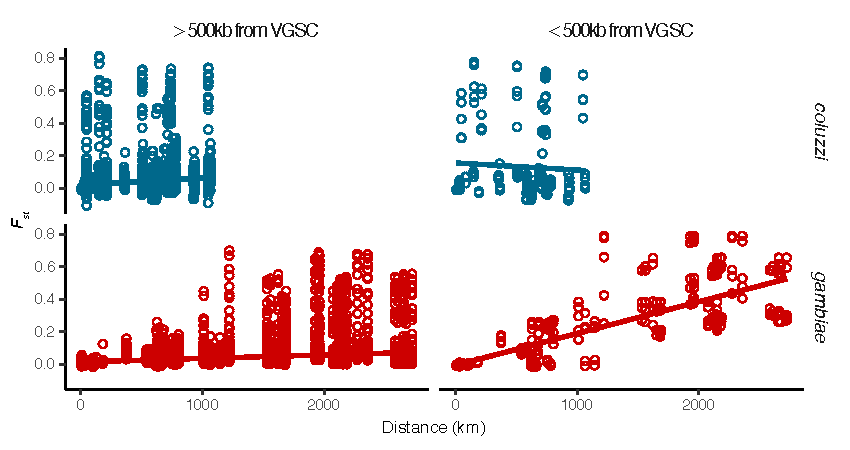
\includegraphics[width=\textwidth]{artwork/fst_by_dist_species_VGSC_edit.pdf}
    \end{center}
    \caption{$F_{st}$ as a function of geographic distance on chromosome 2L at sites more and less than 500kb from \textit{Vgsc}, a gene involved in insecticide resistance. Differentiation of the \textit{Vgsc} regions is strongly related to geographic distance within \textit{An. gambiae}, but not in \textit{An. coluzzii}.}
    \label{fig:vgsc_ibd}
\end{figure}

%% Table S1 - crosses.
%
\afterpage{%
%\clearpage
% N.B., for some reason using \newgeometry causes page number to get dropped from the subsequent page, so disable for now - not needed if using \footnotesize.
\newgeometry{margin=2cm}
\thispagestyle{empty}
\begin{table}[h]
  \normalsize
  \centering
  \begin{threeparttable}

  \caption{
%
\textbf{colony crosses}.
}
  \label{table:colony crosses}
  
\begin{tabular}{lllr}
\toprule
Cross ID & 
Mother Colony & 
Father Colony &
N progeny \\
\midrule

18-5 & Ghana & Kisumu/G3 & 20 \\

29-2 & Ghana & Kisumu & 20 \\

36-9 & Ghana & Mali & 20 \\

37-3 & Kisumu & Pimperena & 20 \\

42-4 & Mali & Kisumu/Ghana & 14 \\

45-1 & Mali & Kisumu & 20 \\

46-9 & Pimperena & Mali & 20 \\

47-6 & Mali & Kisumu & 20 \\

73-2 & Akron & Ghana & 19 \\

78-2 & Mali & Kisumu/Ghana & 19 \\

80-2 & Kisumu & Akron & 20 \\

\bottomrule
\end{tabular}

  \end{threeparttable}

\end{table}
\restoregeometry
} % end afterpage
%% end Table 1

\clearpage


\end{document}
